%  SingleXBs
%  Created by Dave Williams on 2009-06-25.
%  

% header (fold)
\documentclass[]{article}

\usepackage{setspace, float, fancyhdr}
\usepackage[pdftex]{graphicx}
\usepackage[utf8]{inputenc}
\usepackage[round,numbers,sort&compress]{natbib} 
\addtolength{\parskip}{\baselineskip}
\setlength{\parindent}{0in}

% Multi-part figures
%\usepackage{subfigure}
% Package for including code in the document
%\usepackage{listings}

\title{A multidimensional actomyosin cross-bridge model simulates radial forces and the effects of changes in sarcomere lattice spacing} 
\author{C.D.\ Williams, M.\ Regnier, T.L.\ Daniel}
\date{2009--06--25}
% header (end)

\begin{document}

\maketitle{}

\begin{abstract} 
Existing mechanochemical models of muscle contraction assume myosin as a simple linear spring oriented parallel to the direction of the contractile filaments.
Here we describe a model of myosin that closely replicates the force-generating powerstroke by incorporating multiple springs.
This model is based on the protein structure of myosin so that the four springs which comprise it correspond to mechanically relevant portions of myosin's structure.
The behavior of this four spring crossbridge (4sXB) is based on stochastically driven binding and distortion dynamics that are consequences of thermal fluctuations. 
This 4sXB takes most parameters from experimental measurements and permits monitoring of phenomena not possible with a single-spring crossbridge.
The 4sXB generates radial force (orthogonal to the direction of contraction) during its power stroke similar to what a crossbridge produces.
Also, as with a crossbridge, our 4sXB model has binding and state-transition kinetics  and temporal dynamics of force production that vary with lattice spacing. 
 This dependence on lattice spacing follows from changes in angles of attachment  and effective distances. 
Additionally, we describe a simpler two spring crossbridge (2sXB) that replicates most qualities of the 4sXB.
Unlike the 4sXB, the length and angle of the springs comprising the 2sXB can be determined analytically for any chosen head position without the use of iterative techniques.
The forces generated by the 4sXB and the 2sXB are similar.
The rate at which the multi-spring cross-bridges bind and generate force depend on lattice spacing, decreasing as lattice spacing grows. 
The axial and radial forces generated by the multi-spring cross-bridges increase in magnitude as lattice spacing is offset from the myosin head resting position. 
These factors are possible regulators of force production as length and lattice spacing change in the intact muscle.
\end{abstract}

Keywords: myosin; spatially-explicit model; cross-bridge kinetics; lattice spacing

% \paragraph*{Author Summary} % (fold)
% Models of muscle contraction have long treated the molecular motor myosin as a simple spring oriented parallel to its direction of movement. 
% This does not allow for the investigation of phenomena such as the perpendicular force observed during shortening, or the dependence of the maximum force produced on spacing between the contractile filaments that comprise muscle.
% We demonstrate an alternative model, computationally simple enough to use in large networked models, that incorporates both linear and torsional (angle dependent) springs. 
% This model type captures much of the behavior missing from single spring models of the cross-bridge.
% paragraph author_summary (end)


\section{Introduction} %(fold)

% While individual cross-bridges have been treated independently with spatial modeling, thermodynamic accounting has been introduced to the cross-bridge kinetics, compliance introduced to the filaments, and multiple filaments have been arranged to mimic the lattice, the one dimensional nature of the cross-bridge has continued to be used as a model of the mechanism of force generation.

Radial forces are reported to be of the same order as axial forces in contracting muscles \citep{Cecchi1990, Millman1998}. 
In addition, these forces, and radial lattice spacing, are thought to be key determinants of muscle force generation \citep{Fuchs2005}. 
At the same time, structural information about myosin cross-bridges suggests that force is generated through the action of a lever arm \citep{Rayment1993, Uyeda1996, Huxley2000}.
That lever arm generates the strain accompanying the power stroke via a change in the rest angle at which the lever is attached to S1 region \citep{Huxley2000, Houdusse2001}. 
This change in angle occurs at the converter region, a flexible area that acts as a torsional or angular spring. 
\citet{Schoenberg1980b} suggested that these phenomena are related, i.e.\ that radial forces during force generation by a cross-bridge are a result of the geometry of the lever arm. 

Existing theoretical and computational models of cross-bridge force generation, at the level of myofilaments, have assumed force is generated by a simple linear spring oriented parallel to the long axis of the myofilaments.  
This has been the case from the earliest fundamental models of muscle contraction, \citet{Huxley1957}, to more elaborate and spatially explicit models \citep{Daniel1998, Chase2004, Tanner2007}.  
%cite Majailovich ... ????

In the development of computational models of muscle contraction, less attention has been paid to radial forces. 
Thus, the geometry of the single spring cross-bridge has remained largely unchanged while the kinetics underlying transitions between force generating states have increased in complexity throughout subsequent work \citep{Pate1989, Daniel1998, Tanner2007}.
Meanwhile, myosin's lever arm mechanism of force generation suggests that inclusion of torsional springs in computational models would create a system that better reflects the underlying mechanisms of the powerstroke. 
Thus the presence of radial forces along with well established concepts of lever-arm actions of cross-bridges suggest alternate modeling approaches may be appropriate.

Here we examine two models of cross-bridges based on torsional springs.  
Both lend themselves to spatially explicit models of the half sarcomere. 
The first models the cross-bridge as a system of  four linearly elastic springs (4sXB) arranged in a geometry based upon the structure of the S1 and S2 regions of myosin II (Fig.~\ref{fig_xb_types}D). 
Our second model, consisting of two linearly elastic springs (2sXB), replicates many of the behaviors of the 4sXB but provides greater computational efficiency (Fig.~\ref{fig_xb_types}C). 
We use a three-state model of the cross-bridge cycle, consisting of an unbound state, a weakly bound state, and a strongly bound state following a power stroke. 
The kinetics of the three state cycle are similar to those used in previous models \citep{Pate1989, Daniel1998, Tanner2007}, but are generalized to be independent of a model's number of springs.
We quantify both axial and radial forces produced by these model cross-bridges and examine the dependence of such forces on lattice spacing.
In addition, we look at how altering lattice spacing shifts the kinetics (i.e.\ rates of binding, powerstrokes, and cross-bridge detachment) axially, towards the base of the cross-bridge. 

% I killed the next two paragraphs....   merely because they are conjecture and not appropriate for the intro.
%The cross-bridge models developed here, when included in spatially explicit multi-filament models of the half-sarcomere, will permit such models to investigate the effects of radial forces and lattice spacings for the first time. 

% section introduction (end)


\section{Methods}  % (fold)

Our two cross-bridge models, the 4sXB and the 2sXB (Figs.~\ref{fig_xb_types}C-D), are designed to capture a range of mechanical behaviors suggested by the literature.  
Both are based on an arrangement of linearly elastic torsional and Hookean springs.  

\subsection*{Geometry} % (fold)

\paragraph{Spring configurations} % (fold)
For comparison to previous modeling efforts we deploy a simple cross-bridge model consisting of a linearly elastic spring oriented parallel to the long axis of the thick filament (1sXB).  
Forces generated by this cross-bridge are solely oriented in the direction of shortening (axially oriented). 
This 1sXB model is identical to those used in current spatially-explicit computational analyses \citep{Daniel1998, Chase2004, Tanner2007}. 
The one-dimensional 1sXB model cannot, by definition, yield radial forces.  
Moreover, there is no overt mechanism by which this model can account for any dependence on lattice spacing of force or kinetics.

Our four-spring cross-bridge (4sXB) uses two linear and two torsional springs to represent the myosin head (Fig.~\ref{fig_xb_types}D).
This arrangement closely corresponds to regions of the cross-bridge that are thought to be potential domains for strain or deformation. 
In particular, the four springs correspond to the point where the S2 region attaches to the rod, the S2 region, the point where the S2 region attaches to the light chain domain (LCD), and the LCD. 
The torsional spring at the S2/LCD attachment point mimics the action of force generation by change in the angle about the converter region \citep{Houdusse2000, Houdusse2001}. %  TODO : Tom sez re-write this section to name each spring specifically in the figure and relate each named one to the verbiage here.
Since the angle at which the head attaches to actin remains unchanged in our model, the torque generated at the converter region can be accounted for in a torsional spring on the end of LCD linear spring closer to the thick filament attachment point \citep{Lauzon2001}. % TODO : Closely read Lauzon2001 
This multi-spring model of the cross-bridge allows us to compute radial forces and other crossbridge properties that are not present in the 1sXB's one-dimensional space. 
The rest angle of the torsional spring linking the S2 domain and the LCD simulates the power stroke by increasing during the transition from a weakly bound to a strongly bound state.
This method of force generation is acting in two dimensions and thus allows us to include the role lattice spacing plays in determining the cross-bridges' forces and state transition rates.

The 2sXB is a simplification of the 4sXB and uses one linear and one torsional spring to represent the myosin head, (Fig.~\ref{fig_xb_types}C).
In this model, there is still a lever arm mechanism generating force.  
Moreover, we adjusted the length of the lever arm so that the distance from the thick filament to the tip of the cross-bridge is identical to that associated with the 4sXB.
The parameters characterizing the 2sXB are chosen to match the step size, tip location and kinetics of the 2sXB to those of the 4sXB. 
The resulting 2sXB is computationally simpler than the 4sXB, but retains the 4sXB's two-dimensional behavior.

Parameters for both cross-bridges are derived, where possible, from existing experimental data.  
Each linear spring (one in the 1sXB, two in the 4sXB and one in the 2sXB) requires a rest length and spring constant, while each torsional spring (two in the 4sXB and one in the 2sXB) requires a rest angle and spring constant.
The lengths and angles of the springs used for the 4sXB are based on tomographic reconstructions of in vivo S2 lengths and x-ray crystallographic reconstructions of the S1 fragment \citep{Taylor1999, Rayment1993}.
The rest length and angle of the 2sXB are set so that the tips of the 2sXB and 4sXB are in the same location before and after the powerstroke.
% TODO : Please  state the exact numbers and how you got them.    Merely saying they are chosen is tough... 

% Should include a bit on spring constant derivation from Pi hydrolysis energies 
% Consider including a table of parameter values?

%\begin{tabular}
% Parameter     & Value     & Source
% 4sXB          &           & 
% Thick filament/S2 angle 40$^\circ$ 
% S2 spring length 10.5nm Liu et al, 2006
% S2/LCD spring angle
% LCD spring length
% 2sXB          &           & 
% Radial spring length
% Torsional spring angle pre-powerstroke
% Torsional spring angle post-powerstroke
%\end{tabular}
% paragraph spring_configurations (end)

\paragraph{Calculation of lattice spacing} % (fold)
The $d_{1,0}$ spacing is derived from the geometry of the cross-bridge and the lattice spacing having the smallest radial force. 
The multi-spring model provides a measurement of spacing that is analogous to the in vivo surface-to-surface distance between the thick and thin filaments.
The $d_{1,0}$ spacing is calculated from this surface-to-surface lattice spacing (ssLS) using a correction factor for $d_{1,0}$ being measured from the center of one thick filament to the center of another. 
Specifically, $d_{1,0}$ is given by $d_{1,0} = 1.5 (ssLS + cf)$. % TODO : Try a rewrite of this paragraph with this at the front and the rest as an explanation.
The correction factor used to calculate $d_{1,0}$ is determined by designating the resting ssLS of a cross-bridge in the post-power stroke state as having neither compressive nor tensile radial forces. 
This offset becomes 6.90 nm when the rest $d_{1,0}$ spacing is 34 nm \citep{Brenner1991}. 
The ssLS that correspond to the range of extreme $d_{1,0}$ spacings are then calculated and used to define the window of lattice spacings we examine \citep{Millman1998}. % TODO : This could be better if it had more references to ``typical'' lattice spacing papers
Thus the rest ssLS in the model, the lattice spacing at which radial forces are minimal and the geometry of the actomyosin lattice are sufficient to parameterize how lattice spacing is defined for modeled crossbridges. 
% paragraph calculation_of_lattice_spacing (end)

\paragraph{Displacement and force generation} % (fold)
Based on earlier mechanical models of force generation \citep{Pate1989, Daniel1998, Tanner2007} each cross-bridge undergoes a distortion upon the hydrolysis of ATP to ADP.P$_i$.  
That distortion changes the effective rest length of the cross-bridge by an amount proportional to the energy derived from the hydrolysis.  
Within the 1sXB, this distortion is accomplished by a change in the rest length of the cross-bridge's spring. 
In the 4sXB and 2sXB that distortion lies in a change of the rest angle of a torsional spring, a process more closely replicating the lever-arm mechanism \citep{Reedy2000}.
The distortional strain energy liberated by the release of P$_i$ drives force generation by the cross-bridge, appearing as a change in the cross-bridge's rest length.  
The force generated by this process has both axial and radial components. 
The axial component of a vector such as force is the portion that lies along the thick and thin filaments' long axes. 
The radial component of a force vector lies perpendicular to the thick and thin filaments, orthogonal to the axial component. 
The relative values of the post-powerstroke axial and radial forces are determined by the cross-bridge's geometry and the location at which the cross-bridge tip is bound. 
% paragraph displacement_and_force_generation (end)

\paragraph{Calculation of spring lengths and angles} % (fold)
% TODO : This paragraph is terrible, rewrite it.
% Goal here is to clearly communicate the ways in which the spring components are calculated. This should go through: what each angle actually is (from where to where with what as the apex), calculation of angle for 4sXB, and calculation of angle for the 2sXB.
When the 1sXB is placed under strain such that the myosin head is horizontally offset from the thick filament attachment site relative to its resting position, the length of the 1sXB's spring is simple to find as it must completely span the head to thick filament attachment distance.
The lengths and angles of the springs in the 2sXB and 4sXB must take into account the radial distance they must cover as well.
The 2sXB may be analytically determined, as it has all spring values set by the choice of a head location, with arm length and angle given by $r(h_x, h_y)=(h_x^2 + h_y^2)^{1/2}$ and $\theta(h_x, h_y)=\arctan(h_y/h_x)$, respectively.
The 4sXB's increased degrees of freedom require iterative optimization to find the location of the distal torsional spring representing the link between the S2 and S1 regions when the cross bridge's head is moved to a new location.
We use a modification of Powell's ``dog-leg'' method (from \citet{SciPy}) to relax the location of the distal torsional spring to that which results in the lowest energy state of the 4sXB.
Once the distal torsional spring's location is known (as $(c_x, c_y)$), the angle of the proximal torsional spring and the lengths of the two linear springs are determined analytically.
The angle of the proximal torsional spring is given as $\phi(c_x, c_y)=\arctan(c_y/c_x)$, the length of the proximal linear spring as $\ell(c_x, c_y)=(c_x^2 + c_y^2)^{1/2}$, the angle of the distal torsional spring as $\theta(c_x, c_y, h_x, h_y) = \arctan((h_y-c_y)/(h_x-c_x)) + \pi - \phi(c_x, c_y)$, and the length of the distal linear spring as $r(c_x, c_y, h_x, h_y)=((h_x-c_x)^2 + (h_y-c_y)^2)$.
% paragraph calculation_of_spring_lengths_and_angles (end)
% subsection geometry (end)

\subsection*{Kinetics} % (fold)

We use a simplified three state model of the cross-bridge cycle \citep{Pate1989, Tanner2007}. 
This simplified system directly links the cross-bridge's kinetics to mechanics; the three kinetic states are directly comparable to the myosin configurations described in \citet{Houdusse2000}.
The three states represented in our kinetics are (1) an unbound state: Myosin-ADP-P$_i$ (2) a loosely-bound state:Actin-Myosin-ADP-P$_i$ and (3) a tightly-bound force-generating state: Actin-Myosin-ADP (Fig.~\ref{fig_xb_types}A).

The kinetics of both the two spring and the four spring models are strain dependent and are essentially transforms of the free energy landscapes experienced by the cross-bridges in their different states.
These free energies are a function of the distortion necessary to move the point representing the cross-bridge's head to the point where we presume a binding site to be.
Examples of these free energy landscapes are shown in figures \ref{fig_kinetics_contours}A and \ref{fig_kinetics_contours}B, with cuts through them at the rest lattice spacing visible in figure \ref{fig_kinetics_cuts}A.

The binding of both the two and four spring cross-bridges is determined by Monte-Carlo simulation of their diffusion as a result of being perturbed by Boltzmann derived energy distributions \citep{DillBook}. 
After a new head location is found, a binding probability is calculated that decreases exponentially with distance from the potential binding site. 
This probability is tested against a random number from a uniform distribution to determine if binding occurs.

\paragraph{Free energy in each state} % (fold)
The total energy (liberated by the hydrolysis of the gamma P$_i$ of ATP) available to a cross-bridge depends on the concentrations of $ATP$, $ADP$ and $P_i$ and is given by $\Delta G = -\Delta G_{0,ATP} - \ln \frac{[ATP]}{[ADP] [P_i]}$. 
In weakly and strongly bound states a portion of that energy is available to the cross-bridge, allowing the cross-bridge at most 28\% (in the weakly bound state) or 68\% (in the strongly bound state) of $\Delta G$ for mechanical work (see efficiency factors $\alpha=0.28$ and $\eta=0.68$ below; \citet{Pate1989, Tanner2007}).
The total free energy of a cross-bridge in each state also depends on the strain the cross-bridge experiences from distortion upon binding.
Thus the total free energy is a linear combination of the strain-dependent and phosphate-dependent energy of the cross-bridge in each state.
The free energy of the 4sXB system in each state is: 
%Energy of the four spring cross-bridge
\begin{eqnarray}
\label{4sEnergy}
U_1(\phi,\ell,\theta,r) & = & 0 \nonumber \\
U_2(\phi,\ell,\theta,r) & = & \alpha \Delta G + \frac{k_\phi (\phi-\phi_0)^2 + k_\ell (\ell-\ell_0)^2 + k_\theta (\theta-\theta_0)^2 + k_r (r-r_0)^2}{2} \nonumber \\
U_3(\phi,\ell,\theta,r) & = & \eta \Delta G + \frac{k_\phi (\phi-\phi_0)^2 + k_\ell (\ell-\ell_0)^2 + k_\theta (\theta-\theta_1)^2 + k_r (r-r_0)^2}{2} \nonumber
\end{eqnarray}
The free energy of the 2sXB system in each state is: 
% Energy of the two spring cross-bridge
\begin{eqnarray}
\label{2sEnergy}
	U_1(r,\theta) & = & 0 \nonumber \\
    U_2(r,\theta) & = & \alpha \Delta G + \frac{k_r (r - r_0)^2 + 
                        k_\theta (\theta - \theta_0)^2}{2} \nonumber \\
    U_3(r,\theta) & = & \eta \Delta G   + \frac{k_r (r - r_1)^2 + 
                        k_\theta (\theta - \theta_1)^2}{2} \nonumber
\end{eqnarray}
% paragraph free_energy_in_each_state(end)

\paragraph{Binding rate calculation} % (fold)
Our binding algorithm is descended from \citet{Tanner2007} but differs in two key ways: we treat binding as a two step process and our diffusion step works with any number of springs.
Binding depends on diffusion of the cross-bridge head and proximity to the nearest binding site.
Analogously, the process we use to simulate binding has two components, first the diffusion of the myosin head to a new location and then possible attachment to the nearest binding site (depending on the distance from the head and the binding site).
The first step, diffusion, is simulated by thermally forcing each of a cross-bridge's constituent springs with an energy given by a Boltzmann distribution \citep{BergBook, HowardBook}.
This translates to assigning each spring a length or angle chosen from the probability density function $P(x) = \sqrt{k / (2 \pi kT)} \exp^{-(k x^2)/(2 kT)}$ where $x$ is the offset, $k$ is the spring constant of the spring under consideration, and $T$ is the system's temperature in Kelvin  \citep{DillBook, HowardBook}.
We find the updated location of the cross-bridge head from these new spring lengths and angles.
% Probability of binding based on distance to binding site
The probability the cross-bridge will form an attachment depends on the exponential of $d$, the distance from the cross-bridge head's new location to the nearest binding site.
Specifically, the probability of attachment is given by $p_{12}(d) = \gamma \exp ^{d}$, where $\gamma$ is a scaling factor chosen to provide attachment rates consistent with previous estimates.
Attachment occurs if $p_{12}$ is greater than $rand$, a number between 0 and 1 chosen from a uniform distribution \citep{Tanner2007}.
This process is used to determine whether a cross-bridge binds during a single timestep; binding rates are calculated as the fraction of an ensemble of cross-bridges that bind given the same starting conditions. 
Thus, for an ensemble of size $n$: 
$$r_{12} =  \frac{\sum_0^n \left( 1\; \textrm{if}\; \gamma \exp^{-d}>rand ,\; \textrm{else}\; 0 \right)}{n}$$
This two step system, with diffusion followed by a chance of attachment, is used for both the 4sXB and 2sXB with only a change in the number of thermally forced springs.
% paragraph binding_rate_calculation (end)

\paragraph{Powerstroke and detachment rates} % (fold)
% TODO : Consider siphoning off the constants as variables.
The powerstroke and detachment rates are based on prior models but  generalized here for the 4sXB and 2sXB in two-dimensional space by writing them in terms of a dependence on the free energy of the cross-bridge  \citep{Pate1989, Tanner2007}. 
Both the powerstroke rate, $r_{23}$, and the detachment rate, $r_{31}$, are distortion dependent as they depend on the differences in free energy between the current state and the one being considered for transition. 
This means that transitions are more likely when they are energetically favorable and less likely in other circumstances, a natural scheme based in the geometry of the cross-bridges.
The particular rates are as follows for both the 4sXB and the 2sXB: % TODO : Update constants.
$$r_{23}(U_2, U_3) = 1 + 500 * (100 + 1000 \tanh(0.6 (U_2 - U_3))) $$
$$r_{31}(U_3, U_1) = 1000\sqrt{0.01 *  (U_3 - U_1)} + 20$$
% paragraph unbinding_rate (end)

\paragraph{Calculation of reverse rates} % (fold)
% TODO : Fix up this paragraph with a nice ending covering exactly how the reverse transition from bound to unbound will be calculated.
Reverse transition rates are given by the thermodynamically balancing formula $r_{ij}/r_{ji}=\exp^{U_i-U_j}$ where $r_{ji}$ is the forward rate and $r_{ij}$ is the reverse rate \citep{Pate1989, Daniel1998, Tanner2007}.
For the transition from a weakly bound state to an unbound state this requires that the reverse transition is again treated as a fraction of an ensemble of transition opportunities. 
% paragraph calculation_of_reverse rates (end)
% subsection kinetics (end)

% section materials_and_methods (end)


\section{Results} % (fold)

% Intro paragraph (fold)
The 4sXB and 2sXB models detailed here were developed to examine consequences of lattice spacing on cross-bridge kinetics and two dimensional force production.
Multi-spring cross-bridges introduce lattice spacing dependence into force production and kinetics, and account for radial forces not aligned with the direction of contraction. 
As lattice spacing changes, the kinetics and forces of the 4sXB and 2sXB shift in both magnitude and axial offset.
% Intro paragraph (end)

\paragraph{At 34 nm $d_{1,0}$, the multi- and single-spring cross-bridges have similar kinetics and energies} % (fold)
The characteristics of the multi-spring cross-bridges are similar, at their rest lattice spacing of 34 nm $d_{1,0}$, to those of the 1sXB.
In Figure \ref{fig_kinetics_cuts} we compare the free energy, binding rates, powerstroke rates and detachment rates of the multi-spring crossbridges to data from the 1sXB as calculated in \citet{Tanner2007}. 
This similarity is retained from the common basis of the multi- and single-spring cross-bridges' kinetics \citep{Pate1989}.
The cross-bridge properties of the 1sXB, 2sXB and 4sXB are shown together in figure \ref{fig_kinetics_cuts}, where the 1sXB values used are calculated as in Figure 10 of \citet{Tanner2007}. 
Although the properties of the multi- and single-spring cross-bridges are largely similar, some divergences are seen. 
The free energies of the multi-spring cross-bridges are the products of springs at different angles and so are slightly skewed from the symmetric hyperbola of the 1sXB  (Fig.~\ref{fig_kinetics_cuts}A).
The two-dimensional diffusion-based binding probability function that governs the multi-spring cross-bridges causes their likely binding areas to occupy a greater range of axial positions than those of the single-spring cross-bridge (Fig.~\ref{fig_kinetics_cuts}B and \citet{BergBook, DillBook}).
The multi-spring cross-bridges are thus less likely than the 1sXB to bind at a small offset, but more likely than the 1sXB to bind at larger offsets. 
This spread of binding regions reflects the increase in degrees of freedom present in the two-dimensional cross-bridges. 
The powerstroke rates of the multi-spring cross-bridges are essentially those of the single-spring cross-bridge, with energy dependent terms now using the  sum of the free energy of every spring comprising a cross-bridge  (Fig.~\ref{fig_kinetics_cuts}C). 
The detachment rate of the 1sXB explicitly relies on cross-bridge position as well as energy; the dependence on position was removed in adapting the detachment rate for the multi-spring cross-bridges. 
The detachment rate thus loses the intentional asymmetry that the position term provided and retains only the asymmetry created by the spring geometries of the 2sXB and 4sXB (Fig.~\ref{fig_kinetics_cuts}D). 
Thus the detachment rate, like the other cross-bridge properties, maintains the greatest similarity to the 1sXB consistent with the proposed changes: embedding the cross-bridge in multiple dimensions and the transition to generalized kinetics based on cross-bridge free energy. 
% paragraph (end)

\paragraph{Axial offset of most cross-bridge properties decrease as lattice spacing increases} % (fold)
The axial offset of most energies and kinetics of the 4sXB and 2sXB decreases as lattice spacing grows larger.
The axial offset of a cross-bridge property is the distance from the thick filament attachment site to that property's extreme value or point of inflection at a given lattice spacing. 
An example of this change in axial offset is visible in Figures \ref{fig_kinetics_contours}A-B where the lowest energy point that the 4sXB or the 2sXB may reach at a lattice spacing of 32 nm $d_{1,0}$ is more than 3 nm further from the cross-bridge's thick filament attachment point than the lowest energy point reachable at a lattice spacing of 38 nm $d_{1,0}$.
This relationship between axial offset and lattice spacing changes the behavior of a cross-bridge as lattice spacing grows or shrinks.
Since binding at a large axial offset is unlikely to occur at a larger lattice spacing, forward biasing of binding is decreased with increases in lattice spacing (Figs.~\ref{fig_kinetics_contours}C-D). 
Similarly, decreases in the axial offset of the powerstroke rate's inflection point as lattice spacing increases causes the size of the powerstroke to change with lattice spacing (Figs.~\ref{fig_kinetics_contours}E-F).
The detachment rate of the 4sXB is the only cross-bridge property where the axial offset does not decrease as lattice spacing increases (Fig.~\ref{fig_kinetics_contours}G).
This is due to the radially aligned post-powerstroke orientation of the 4sXB's final linear spring. 
Combined, these effects reduce the axial force a cross-bridge generates at larger lattice spacings with implications for the sarcomere length dependence of force production and relaxation. 
% paragraph (end)

\paragraph{Probability of a cross-bridge being bound decreases as lattice spacing diverges from rest} % (fold)
As lattice spacing diverges from its 34 nm $d_{1,0}$ rest value, the attachment rate baseline decreases while the detachment rate baseline increases, making the number of cross-bridges in a force generating state dependent on lattice spacing (Figs.~\ref{fig_kinetics_contours}C-D and \ref{fig_kinetics_contours}G-H). 
The baseline of a cross-bridge property is its magnitude across all axial offsets, the offset of that property's value from zero. 
These kinetic rate baselines change with lattice spacing because the energy differential, on which they depend, increases with lattice spacing.
Binding and detachment rates are dependent on the difference in free energy between the unbound state and the weakly bound state in the first case and between the tightly bound state and the unbound state in the second.
As above, the rest lattice spacing is defined by the radial offset at which multi-spring cross-bridges under no strain come to rest. 
Thus, as the lattice spacing increases or decreases from the point where bound cross-bridges are under the least strain, the energy difference between a bound state and the zero-energy unbound state increases. 
This increase in energy makes the cross-bridge increasingly likely to transition to the unbound state and remain there (Figs.~\ref{fig_kinetics_contours}C-D and  \ref{fig_kinetics_contours}G-H). 
An example of this can be seen in that the slowest detachment rate of the 4sXB is 20/sec at a lattice spacing of 34 nm $d_{1,0}$ while at 38 nm $d_{1,0}$ the minimum detachment rate is 260/sec (Fig.~\ref{fig_kinetics_contours}G).
In models incorporating multiple cross-bridges, the dependence of kinetic rates on lattice spacing decreases the chance a cross-bridge will generate force as lattice spacing increases. 
This is one factor regulating the force a lattice generates as length and lattice spacing change during contraction.
As lattice spacing is compressed below rest, cross-bridge induced realignment of binding sites due to the greater possible step size of each cross-bridge may cancel this effect.
As the powerstroke rates depend on the difference between $\tanh$ of two parabolic energy profiles, their maximum and minimum probabilities of a cross-bridge undergoing a powerstroke do not change with lattice spacing (Figs.~\ref{fig_kinetics_contours}E-F). 
Individual cross-bridges spend less time in a bound state as a result of these changes in their kinetics as lattice spacing diverges from its rest value.
% paragraph (end)

\paragraph{Forces at a given axial offset increase with lattice spacing} % (fold)
The axial and radial forces at a given axial offset increase as lattice spacing grows larger.
The force a cross-bridge produces trend from initial negative values at compressed lattice spacings, through spacings where little force is produced, to very positive values at expanded lattice spacings (Figs.~\ref{fig_forces}E-H). 
This effect competes with the decreased rate of binding and force generation that a multi-spring cross-bridge experiences at greater lattice spacings. 
At large lattice spacings few cross-bridges will generate force, but those that do will generate more per cross-bridge. 
An increase in forces with lattice spacing is seen, for example, where the 4sXB at 10 nm axial offset and 35 nm $d_{1,0}$ gives half the axial and half the radial force as the same cross-bridge at 38 nm $d_{1,0}$ (Figs.~\ref{fig_forces}E,G). 
Similarly, a 2sXB at 12 nm axial offset and 35 nm $d_{1,0}$ gives about two thirds of the axial and radial forces as at 38 nm $d_{1,0}$ (Figs.~\ref{fig_forces}F,H).  
These energy landscapes also show that no lattice spacing is free of radial force across all axial offsets.  
The radial force produced by a cross-bridge, even at rest lattice spacing, increases in magnitude as the cross-bridge tip moves away from its unstrained axial offset. 
While the forces of both the 4sXB and the 2sXB undergo similar trends of increasing forces with lattice spacings, the details of their force landscapes differ as a result of their different spring geometries (Fig.~\ref{fig_forces}). 
At large lattice spacings, this greater force per cross-bridge is countered by the decreased probability a cross-bridge will generate force, an interaction requiring a model of the half-sarcomere using the 2sXB or 4sXB to evaluate throughly \citep{Martyn2004}. 
% paragraph (end)

\paragraph{Radial forces are of the same order of magnitude as axial forces} % (fold)
The radial and axial components of force, produced by a 4sXB or 2sXB moved from its rest position to an axial offset, are of the same order of magnitude (Figs.~\ref{fig_forces}A-D). 
The 2sXB and 4sXB are the first models of the cross-bridge, suitable for use in larger spatially explicit simulations of the half sarcomere, to be capable of monitoring experimentally demonstrated radial forces \citep{Cecchi1990, Millman1998}. 
The relative values of the radial and axial forces are visualized as the angles of the force vectors in Figures \ref{fig_forces}A-D. 
Axial locations and lattice spacings with balanced axial and radial forces produce force vectors that are neither vertical nor horizontal, but in some middle orientation.
Most axial and radial offsets are populated by such vectors, particularly areas which a cross-bridge is most likely to occupy (indicated by shading, with the darkest arrows being the most likely locations). 
The few areas that are dominated by one force, notably some small offset positions of the 2sXB (Fig.~\ref{fig_forces}D), are dominated by radial forces.
This strong presence of radial forces suggests that in all but the least strained locations, radial forces will be present in magnitudes similar to those of axial forces. 
Thus multi-spring cross-bridges will make it possible to evaluate the influence of these radial forces, posited to be regulators of axial forces and the relationships such as the Frank-Starling mechanism; something not possible with a 1sXB. 
% paragraph (end)

% section results (end)


\section{Discussion} % (fold)

 %  * Provides new cross-bridge mechanics for use in models
 %   - Comparison to single spring system
 %   - Low computational requirements of 2s cross-bridge
 %   - Possible: balancing radial forces with multiple filaments
 %  * No longer depends on strained binding, moving towards non-ratchet
 %   - 1s is rectification based as in refs 1,2 of Davis & Epstein 2009
 %   - Both 2s & 4s allow a power stroke mechanism (recalc spring consts)
 %  * Axial forces compared to experimental data
 %   - Comparison Schoenberg work (TNCG/xxCG versus xNxx/xNCx)
 %   - Ask M+T what experimental work would be good to compare to
 %   - Comparison to dextran LS compression and force levels? Probably not.
 %  * Radial forces and experimental observations of compression (Cecchi)
 %   - Check magnitude of forces needed

% Discussion intro paragraph %(fold) 
This work shows that a multi-spring cross-bridge can effectively model both lattice spacing dependence and radial force production. 
The 4sXB and 2sXB demonstrate that several properties, such as varying step size with changes in lattice spacing, emerge when a torsional spring and a lever-arm mechanism are used to generate force. 
The radial forces produced by this lever-arm mechanism were of the same magnitude as the axial forces, a ratio similar to that observed experimentally \citep{Cecchi1990,Brenner1991}. 
These cross-bridge models are the first to make such comparisons.
The newly modeled dependencies of step-size and binding likelihood on lattice spacing have the potential to explain differences in observed force generation at altered lattice spacings  \citep{Millman1998}. 
These cross-bridge models, designed to investigate radial force and the effects of lattice spacing, should yield further insight into the importance of non-axial dimensions when incorporated into a spatially explicit model. 
% (end)

\paragraph{Force generated by a multi-spring cross-bridge depends on lattice spacing} % (fold) 
A multi-spring cross-bridge's energy landscape, and the resulting force of its powerstroke, depend on the cross-bridge's lattice spacing.
At most locations, the forces a cross-bridge produces at a given axial offset increase as lattice spacing grows and strain on the cross-bridge increases (Fig.~\ref{fig_forces}E-H). 
While this increased strain translates into greater axial and radial force per strongly bound cross-bridge, the binding probability decreases as lattice spacing increases (Fig.~\ref{fig_kinetics_contours}C-D).
The decrease in attachment rate at extreme lattice spacings, while powerstroke rates remain unchanged (Fig.~\ref{fig_kinetics_contours}E-F), suggests lattice spacing influences muscle fiber force generation by altering the rate of cross-bridge attachment rather than the powerstroke rate \citep{Martyn2004}. 
How this decreasing number of bound, force generating cross-bridges translates into less force as lattice spacing increases in the compliant sarcomere (and how closely this will match experimental results) will be determined by incorporating multi-spring cross-bridges into larger, spatially explicit models. % TODO : find a good LS vs max force paper to cite, ask Mike about this 
% paragraph strain_and_force_generation_at_the_level_of_a_single_cross-bridge_depend_on_lattice_spacing (end)

\paragraph{Multi-spring cross-bridge step size varies with lattice spacing} % (fold)
The 4sXB's and the 2sXB's geometry dictates that a change in step size must accompany a change in lattice spacing. 
Step size is defined as the axial distance a myosin head moves between pre- and post-powerstroke angles, if it is unconstrained in the axial direction and allowed to settle into the post-powerstroke position that minimizes the energy stored in the cross-bridge.
Step size changes with lattice spacing because the difference between the pre-powerstroke and the post-powerstroke cross-bridge angle does not vary with changes in lattice spacing while the change in the length of the lever arm does. 
Because the distance subtended by a given angle will increase as lever arm increases, step size will grow as lattice spacing increases. 
This phenomena is more pronounced in the 2sXB, which lacks a second set of springs to help compensate for lattice spacing changes, placing the full burden of bridging the thick and thin filaments on the lever-arm. 
However, the 4sXB possesses a set of springs between the lever-arm and the thick filament.
These additional springs also adjust with lattice spacing, allowing the location of the 4sXB's lever-arm pivot point to change with lattice spacing and decreasing the amount by which the 4sXB's step-size changes with lattice spacing.  
Wether this phenomena is present in physical cross-bridges is unknown, most measurements of step-size have been made in isolated in-vitro preparations that are unable to simulate a change in muscle lattice spacing. % TODO : Cite some step size work.
This factor may alter the force generated at different lattice spacings and the proportion of crossbridge that remain bound after completing a powerstroke; greater step-size will increase the cross-bridge's strain and probability of detachment shortly after powerstroke is completed. 
% paragraph step_size_varies_with_lattice_spacing_for_a_two_spring_cross-bridge (end)

% \paragraph{Lattice spacing alters both likelihood of interaction and likely interaction location} % (fold)
% % paragraph lattice_spacing_alters_both_likelihood_of_interaction_and_likely_interaction_location (end)

% TODO Incorporate the following paragraph into the intro?
% \paragraph{Increased fidelity to known structure and mechanisms} % (fold)
% The multiple spring cross-bridges both have a far greater ability than single spring cross-bridges to replicate the defining characteristics of muscle myosin structure and the lever arm mechanism of force generation. 
% The 2sXB and the 4sXB both generate force through the changing of the rest angle of a torsional spring attached to a lever arm.
% This is closely analogous to the lever arm mechanism as it is understood and stands in contrast to the mechanism by which a single spring cross-bridge replicates the powerstroke \citep{Houdusse2001}.
% The single spring cross-bridge generates its force with an offset of the myosin head can also be thought of as the spring representing the cross-bridge having a different rest length in the unbound state and the loosely bound state than it does in the tightly bound state. 
% This offset or altered rest length is what determines the stroke distance of the single spring cross-bridge and estimates of it have varied from as little as 1 nm to as large as 10 nm (needs citation). 
% By treating the cross-bridge as several components instead of a single spring we are able to base input parameters on values that can be referenced to existing crystallography structures.
% paragraph increased_fidelity_to_known_structure_and_mechanisms (end)

\paragraph{Large radial component of forces may influence lattice spacing in multi-filament models} % (fold) 
The 4sXB and the 2sXB produce large radial forces: forces of the same order of magnitude as the axial forces a cross-bridge generates. 
%These forces range between 10\% and 50\% of the axial force at the axial offsets at lattice spacings where a cross-bridge is most likely to become strongly bound (Fig.~\ref{fig_forces}).
The 4sXB and 2sXB are the first spatially explicit cross-bridge models that are able to model the observed radial component of muscle contraction.
Observations of lattice spacing during redevelopment of tension following length changes provides experimental evidence of strong radial forces at the level of individual muscle fibers \citep{Cecchi1990}. % Cecchi1990 sez radial forces are 23% of axial 
A spatially explicit model, even using multiple thick and thin filaments arranged in a lattice, is insensitive to lattice spacing if it uses a version of the 1sXB.
Embedding the multi-spring cross-bridges in a multi-filament model will allow simulation of radial force regulation in a lattice of thick and thin filaments.  
Radial force has been put forward as a regulator of lattice spacing and of Ca$^{2+}$ sensitivity as lattice spacing and sarcomere length vary; a multi-filament model using the 4sXB or 2sXB can simulate the interaction of cross-bridge generated radial force with restoring forces provided by other mechanisms, e.g.\ titin or electrostatic repulsion \citep{Martyn2004, Cazorla2001}. % TODO : Close read of Cazorla. Add electrostatic paper.
Inclusion of these forces in future modeling efforts will present an opportunity to examine an interaction ignored by previous spatially explicit models and assess its likely contribution to lattice spacing regulation and lattice spacing sensitive processes, such at the Frank-Starling mechanism. % TODO : Justify FSM more?
% paragraph modeled_radial_forces_are_too_large_to_ignore (end)

\paragraph{The 2sXB approximates the 4sXB} % (fold)
The energies, kinetics, and forces generated by the 2sXB are not exact duplicates of those governing the 4sXB, but are subject to the same governing trends (Figs.~\ref{fig_kinetics_contours}, \ref{fig_kinetics_cuts} and \ref{fig_forces}). 
Mimicry of the 4sXB by the 2sXB is intentional and desirable, the 2sXB is intended to be a computationally cheaper alternative to the 4sXB. 
The energies, binding rates, and powerstroke rates of the multi-spring cross-bridges are almost identical, while the rate of detachment is rotated by approximately 20$^\circ$ between the two systems due to differences in the way the post-powerstroke position is achieved (Fig.~\ref{fig_kinetics_contours}).
The greatest differences between the 4sXB and the 2sXB come in the forces that they generate.
The 2sXB requires a 10 nm change in lattice spacing to double the axial force generated at a 10 nm binding site offset, a force increase that takes the 4sXB just under a 6 nm change in lattice spacing (Fig.~\ref{fig_forces}). 
So while both the axial force generated by both cross-bridges depends on lattice spacing, that of the 2sXB does so less than that of the 4sXB.
This pattern is reversed for the radial forces generated by the cross-bridges, where the 2sXB's radial force is more dependent on lattice spacing than is the 4sXB's.
In each of these cases, the forces generated by the each of the multi-spring cross-bridges is subject to the same trend as lattice spacing or axial offset from the binding site increases.
This similarity of forces and near mirroring of energies and kinetics lends support to use of the 2sXB in cases where the 4sXB would be prohibitively computationally expensive.
Ultimately, use of either multiple spring cross-bridge will permit new explorations of the relationships between kinetics, lattice spacing, radial force and axial force.
% TODO: Incorporate the next few lines into materials and methods or intro:
% As discussed above, whenever the head of the 4sXB is moved, the position of the middle torsional spring (roughly equivalent to the converter domain) must be determined iteratively. 
% This imposes a computation cost that is small for a single cross-bridge, but makes longer duration multi-filament simulations require prohibitively large resources. 
% These problems do not exist for the 2sXB which requires no such step.
% As the kinetics and force of the 2sXB system resemble those of the 4sXB system in most instances, with the exceptions of their differing lattice spacing dependencies of the powerstroke rate and precise force orientation at some of the more extreme offsets, it may prove to be a useful model system.
% paragraph simplicity_of_the_2sxb_may_be_desirable (end)


% section discussion (end)


\clearpage
\section*{Figures} % (fold)

\begin{figure}[htbp]
    \begin{center}
    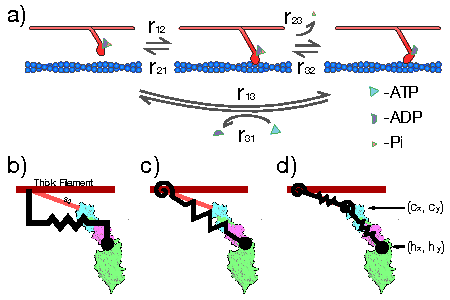
\includegraphics[width=3.2in]{../imgs/Figure1.pdf}
    \caption{
        \label{fig_xb_types}
        \textbf{Kinetic scheme and cross-bridge types under investigation.} 
        The three state kinetic system is shown in subfigure A. 
        The three states represent (1) an unbound state, (2) a weakly bound state, and (3) a strongly bound state. 
        The binding rate ($r_{1,2}$), strong transition rate ($r_{2,3}$), and unbinding rate ($r_{3,1}$) are determined by the energy stored in the springs representing the cross-bridge. 
        The reverse rates ($r_{2,1}$, $r_{3,2}$, and $r_{1,3}$) are functions of the forward transition rates.
        Subfigures B, C, and D show the cross-bridge representations we examine, plotted against a myosin crystal structure for comparison (crystal structure image generated from \citet{Gourinath2003} with MacPyMol). 
        Subfigure B shows the single-spring cross-bridge (1sXB) used heavily used in models since \protect\citep{Huxley1957}. 
        Subfigure C depicts the two-spring cross-bridge (2sXB) which uses both a torsional/angular spring and a linear spring. 
        Subfigure D shows a four-spring cross-bridge (4sXB) using two torsional and two linear springs, which we compare the single and dual spring cross-bridges against. 
        % TODO : Take out the next two lines or make them useful.
        The locations of the distal torsional spring and tip of the 4sXB are denoted as $(c_x, c_y)$ and $(h_x, h_y)$ respectively. 
        The tip of the 2sXB is also denoted as $(c_x, c_y)$.
    }
    \end{center}
\end{figure}

\begin{figure}[htbp]
    \begin{center}
    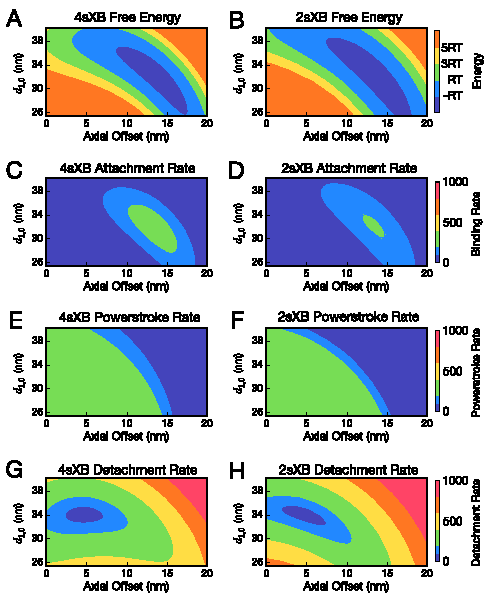
\includegraphics[width=3.2in]{../imgs/Figure2.pdf}
    \caption{
        \label{fig_kinetics_contours}
        \textbf{Energy and kinetics of the 4sXB and 2sXB systems at varying axial offsets and lattice spacings.} 
        Subfigures A through H show the properties of the 4sXB (subfigures A, C, E, and G) and the 2sXB (subfigures B, D, F, and H) as they change with binding site offset and $d_{1,0}$ lattice spacing.
        Binding site offset is the distance between the current axial location of the cross-bridge's tip, $h_x$, and the location where the cross-bridge attaches to the thick filament.
        Lattice spacing ($d_{1,0}$) is defined as in \citet{Millman1998}, with an offset to account for filament thicknesses so that the cross-bridge exactly bridges the two filaments at a rest lattice spacing of 34 nm.
        Subfigure A depicts the free energy of the 4sXB at various lattice spacings (represented along the y-axis), with the head stretched to an axial offset from the thick filament attachment point (zero on the x-axis).
        Similarly, the free energy of the 2sXB is shown in subfigure B.
        The lowest energy myosin head locations in both A and B are shown as the darkest part of the plot and change in axial offset as lattice spacing changes.
        The subfigures C and D show $r_{1,2}$, the probability that the 4sXB and the 2sXB will transition from an unbound state to a bound state, and the dependence of this transition on both the axial offset of the open binding site from the myosin thick filament attachment site and the lattice spacing $d_{1,0}$ which is a function of the distance between the binding site and the thick filament attachment point of the myosin head. 
        Subfigure C depicts this probability for the 4sXB as a two dimensional contour with the same axes as in A while subfigure D depicts the transition probabilities for the two spring cross-bridge.
        Subfigures E and F show $r_{2,3}$, the probability of transition from a weakly bound state to a strongly bound state, for the same cross-bridges, with the same axes and scales as C and D show $r_{1,2}$.
        Subfigures G and H show $r_{3,1}$, the probability of unbinding from a strongly bound state, for the same cross-bridges, with the same axes and scales as C and D show $r_{1,2}$.
        The reverse rates, $r_{2,1}$, $r_{3,2}$, and $r_{1,3}$ may be back-calculated from the forward rates.
    }
    \end{center}
\end{figure}

\begin{figure}[htbp]
    \begin{center}
    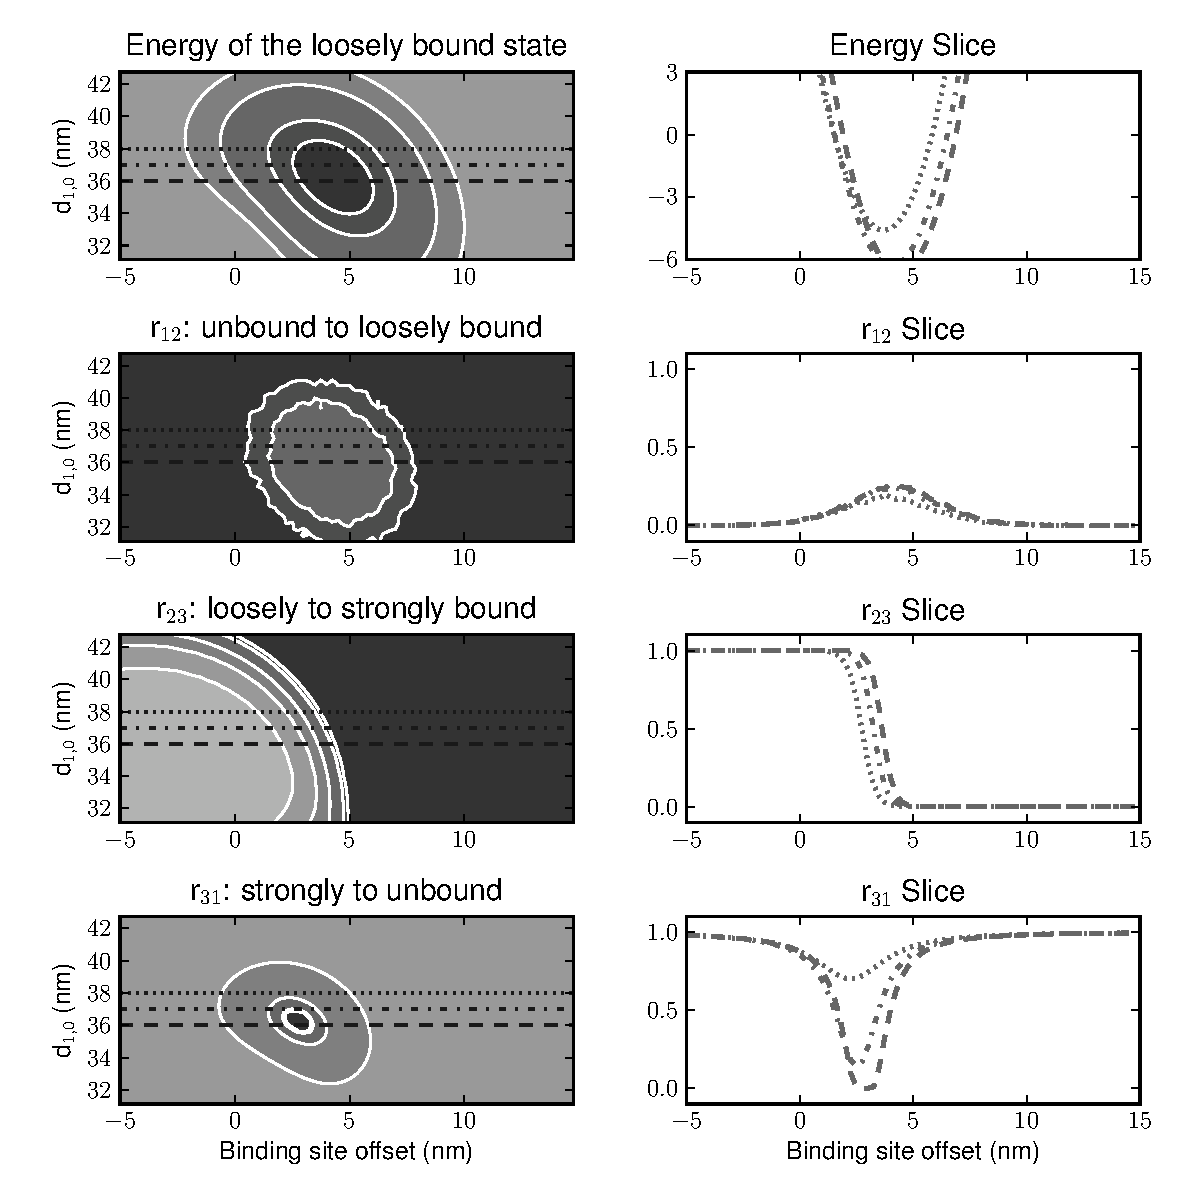
\includegraphics[width=3.2in]{../imgs/Figure3.pdf}
    \caption{
        \label{fig_kinetics_cuts}
        \textbf{Energy and kinetics of the 1sXB, 2sXB, and 4sXB at the resting lattice spacing.}
        Subfigures A through D show the energy and transition rates of the 1sXB (black), 2sXB (green), and 4sXB (red) at resting lattice spacing.
        The 1sXB values shown for comparison are derived from those of \citet{Daniel1998} and \citet{Tanner2007}, shifted axially so the resting location of the cross-bridge head in each case is aligned with that of the 2sXB and 4sXB. 
        The free energy of the cross-bridges in state two is shown in subfigure A, where the multi-spring cross-bridges' shifts from a strictly parabolic trajectory is visible.
        The explicit thermal forcing of the multi-spring cross-bridge heads in subfigure B results in binding probabilities that are more distributed than those of the single spring cross-bridge.
        The rate of powerstrokes, in subfigure C, remains least changed between the single and the multi-spring cross-bridge models.
        The energy-based kinetics of the multi-spring cross-bridges are unable to fully replicate the biased detachment rate of the 1sXB in subfigure D. 
    }
    \end{center}
\end{figure}

\begin{figure}[htbp]
    \begin{center}
    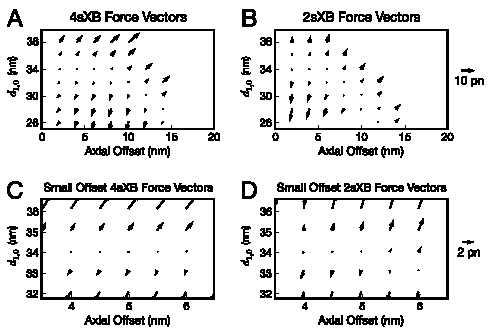
\includegraphics[width=3.2in]{../imgs/Figure4.pdf}
    \caption{
        \label{fig_forces}
        \textbf{Overview and detail of the forces exerted by the 2sXB and 4sXB.}
        Subfigures A through D show the forces exerted by the 4sXB and the 2sXB, with the shade of the vector arrows being determined by the chance of such a configuration occurring, a sum of the $r_{23}$ and the inverse of the $r_{31}$ transition probabilities. 
        Subfigures A and B show overviews of the forces exerted, respectively, by the 4sXB and the 2sXB over lattice spacings and axial offsets that vary as in Figure 2.
        The forces exerted by the two cross-bridges have radial components which frequently equal or exceed their axial components.
        A more detailed view of the region surrounding the rest position of the cross-bridges is shown in subfigures C and D, where the large radial components of the cross-bridge forces, particularly for the 2sXB, is again evident.
        Subfigures E through H show, separated, the axial and radial components of the 4sXB and the 2sXB.
    }
    \end{center}
\end{figure}

% bibliography (fold)
% Bib style requires biophysj.bst be in the document directory
\clearpage
\bibliographystyle{biophysj}
\bibliography{JournalArticles,NotArticles}
% bibliography (end)

\end{document}
